
%---------------------------------------%
% Packages arranged by : Tsz Timmy Chan %
%                 Date : May 26th, 2019 % 
%---------------------------------------%

\documentclass{TC}
\usepackage{TCcommon}

\title{TITLE HERE}	% Work Title Here.
\author{Tsz Timmy Chan}	% YOUR NAME HERE 

\usepackage[notes]{TCheader}
\usepackage{TCexamtitle}

\usepackage{setspace}
\linespread{1.5}

%\renewcommand{\benediction}{" " - }
%\renewcommand{\quoteoftheday}{" " \\ - }

\begin{document}
Theoretical perspectives and Frameworks on How People Learn: Cognitive, Cultural, Sociocultural, Communities of Practice.

Examined the texts How People Learn 1 \& 2 and practiced comparing the two texts in more detail. Got an introduction to the differences between the cognitive and socioculture perspectives on learning and transfer \parencite{sawyer_learning_2014, satyam_cognitive_2018, national_academies_of_sciences_engineering_and_medicine_context_2018, national_academies_of_sciences_engineering_and_medicine_introduction_2018, bransford_design_2000,
bransford_learning:_2000}. Of particular interest is the diagram on perspectives on learning environments \ref{fig:NRC_perspectives_on_learning_enviornment}.

\begin{figure}[h]
\centering
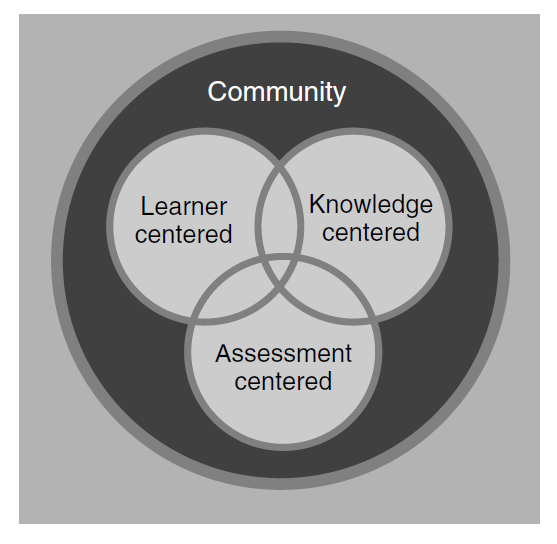
\includegraphics[width=.5\textwidth]{NRC_perspectives_on_learning_enviornment}

\caption{Perspectives on learning enviornments \parencite{bransford_design_2000}.}
\label{fig:NRC_perspectives_on_learning_enviornment}
\end{figure}

\end{document}
